\chapter{Implementacija i korisničko sučelje}
		
		
		\section{Korištene tehnologije i alati}
		
			\textbf{\textit{dio 2. revizije}}
			
			 \textit{Detaljno navesti sve tehnologije i alate koji su primijenjeni pri izradi dokumentacije i aplikacije. Ukratko ih opisati, te navesti njihovo značenje i mjesto primjene. Za svaki navedeni alat i tehnologiju je potrebno \textbf{navesti internet poveznicu} gdje se mogu preuzeti ili više saznati o njima}.
			 
			 Komunikacija u timu realizirana je korištenjem aplikacije \textbf{\href{https://discord.com/}{Discord}}. 
			 Discord je društvena platforma na kojoj korisnici imaju mogućnost komuniciranja tekstualnim porukama, glasovnim
			 pozivima, videopozivima, medijima i datotekama u privatnim porukama ili kao dio zajednice koju nazivaju server. 
			 Za izradu UML dijagrama korišten je alat \textbf{\href{https://www.visual-paradigm.com/}{Visual Paradigm}}. Visual 
			 Paradigm je grafički alat koji omogućava jednostavno modeliranje mnogo različitih tipova UML dijagrama, poput 
			 dijagrama obrazaca uporabe, sekvencijskih dijagrama, dijagrama razreda, dijagrama stanja, dijagrama aktivnosti, 
			 dijagrama komponenata, ERD modela baze podataka i mnogih drugih. Za upravljanje izvornim kodom korišten je 
			 \textbf{\href{https://git-scm.com/}{Git}}. Git je open-source distribuirani sustav za upravljanje različitim 
			 verzijama datoteka. Udaljeni repozitorij projekta je dostupan na web platformi \textbf{\href{https://github.com/}{GitHub}}.
			 GitHub pruža usluge spremanja i upravljanja kodom. Koristi se Git-om kako bi omogućio upravljanje različitim 
			 verzijama datoteka. Također, GitHub omogućava dokumentiranje programske podrške pomoću wiki-ja.

			 Kao razvojno okruženje korišteni su \textbf{\href{https://code.visualstudio.com/}{Visual Studio Code}} 
			 i \textbf{\href{https://www.jetbrains.com/idea//}{Intellij IDEA}}. Visual Studio Code je uređivač teksta
			 razvijen u tvrtki Microsoft. Prvenstveno se koristi za razvoj računalnih sustava na operacijskom sustavu Windows. 
			 Korišten je za razvoj programske podrške na frontendu i razvoj dokumentacije. Intellij IDEA je integrirano razvojno 
			 okruženje (IDE) razvijeno u tvrtki JetBrains. Usmjereno je na razvoj Java aplikacija, no podržava niz drugih jezika i 
			 tehnologija. Korišten je za razvoj programske podrške na backendu.

			 Aplikacija je napisana koristeći radni okvir \textbf{\href{https://spring.io/projects/spring-boot}{Spring Boot}} i jezik 
			 \textbf{\href{https://www.java.com/en/}{Java}} za izradu \textit{backenda} te jezik \textbf{\href{https://www.javascript.com/}{JavaScript}} 
			 i njegovu biblioteku \textbf{\href{https://react.dev/}{React}} za izradu \textit{frontenda}. React je biblioteka 
			 u JavaScriptu za izgradnju korisničkih sučelja. Nastala je od strane Facebooka. Glavna karakteristika Reacta je komponentna 
			 arhitektura, što znači da se korisničko sučelje sastoji od više manjih, ponovno uporabljivih komponenata. Izrada 
			 složenijih aplikacija u Reactu obično zahtijeva korištenje dodatnih biblioteka za interakciju s API-jem. Radni okvir 
			 Spring Boot nudi gotova rješenja i funkcionalnosti koje ubrzavaju razvoj aplikacija. Ima automatsko upravljanje 
			 konfiguracijom i zavisnostima što olakšava i ubrzava posao programerima. Spring Boot pruža podršku za implementaciju 
			 sigurnosti u aplikacijama pomoću Spring Security modula. 

			 Baza podataka izvedena je u \textbf{\href{https://www.postgresql.org/}{PostgreSQL}}-u. PostgreSQL je open-source sustav za upravljanje relacijskim bazama
			 podataka kojim se proširuje funkcionalnost SQL-a. Dizajniran je da izdrži različita radna opterećenja, od 
			 pojedinačnih računala, pa sve do skladišta podataka ili web usluga s mnogo istodobnih korisnika. Baza podataka
			 se na poslužitelju u oblaku \textbf{\href{https://render.com/}{Render}}. Kao okruženje za upravljanje bazom
			 podataka korišten je open-source grafički alat \textbf{\href{https://www.pgadmin.org/}{pgAdmin}}.

		     Dokumentacija je pisana u jeziku \textbf{\href{https://www.latex-project.org/}{LaTeX}}. LaTeX je jezik za pisanje
			 strukturiranih tekstova profesionalne kvalitete. Za razliku od nekih programskih jezika za obradu teksta s grafičkim
			 sučeljem poput Microsoft Worda, dokumenti u LaTeX-u pisani su kao obični tekst s dodanom semantičkom strukturom. Time 
			 postiže usredotočenost na sadržaj, ujednačenost izgleda te brži i stabilniji rad.

			\eject 
		
	
		\section{Ispitivanje programskog rješenja}
			
			\textbf{\textit{dio 2. revizije}}\\
			
			 \textit{U ovom poglavlju je potrebno opisati provedbu ispitivanja implementiranih funkcionalnosti na razini komponenti i na razini cijelog sustava s prikazom odabranih ispitnih slučajeva. Studenti trebaju ispitati temeljnu funkcionalnost i rubne uvjete.}
	
			
			\subsection{Integracijsko testiranje}
			\textit{Potrebno je provesti ispitivanje jedinica (engl. unit testing) nad razredima koji implementiraju temeljne funkcionalnosti. Razraditi \textbf{minimalno 6 ispitnih slučajeva} u kojima će se ispitati redovni slučajevi, rubni uvjeti te izazivanje pogreške (engl. exception throwing). Poželjno je stvoriti i ispitni slučaj koji koristi funkcionalnosti koje nisu implementirane. Potrebno je priložiti izvorni kôd svih ispitnih slučajeva te prikaz rezultata izvođenja ispita u razvojnom okruženju (prolaz/pad ispita). }
			
			Na backendu integracijsko testiranje se sastoji od pozivanja API-a i očekivanja određenog odgovora za taj API.
            Na taj način se testira stvarna procedura koja se odvija kada korisnik pozove taj API.
			Prolazi se kroz sve slojeve backenda - od kontrolera do baze.
			Postoji sveukupno 6 integracijskih testova - 5 njih za modele koji reprezentiraju entitete u bazi te jos jedan za registraciju i prijavu korisnika.
            Integracijski testovi funkcioniraju na način da se prvo u dockeru podigne baza podataka, što se može vidjeti na slici \ref{fig:IT_docker}.
            Nakon toga izvršava se funkcija koja je anotirana sa @BeforeEach anotacijom. 
			Funkcija koja ima anotaciju @BeforeEach će se izvršiti prije svakog testa.
            Također, postoji i funkcija koja je anotirana sa @AfterEach anotacijom. 
			Ona će se izvršiti poslije svakog testa.
            Sami testovi su anotirani sa anotacijom @Test.
			Sve navedene anotacije pripadaju org.junit biblioteci.
            \begin{figure}[H]
                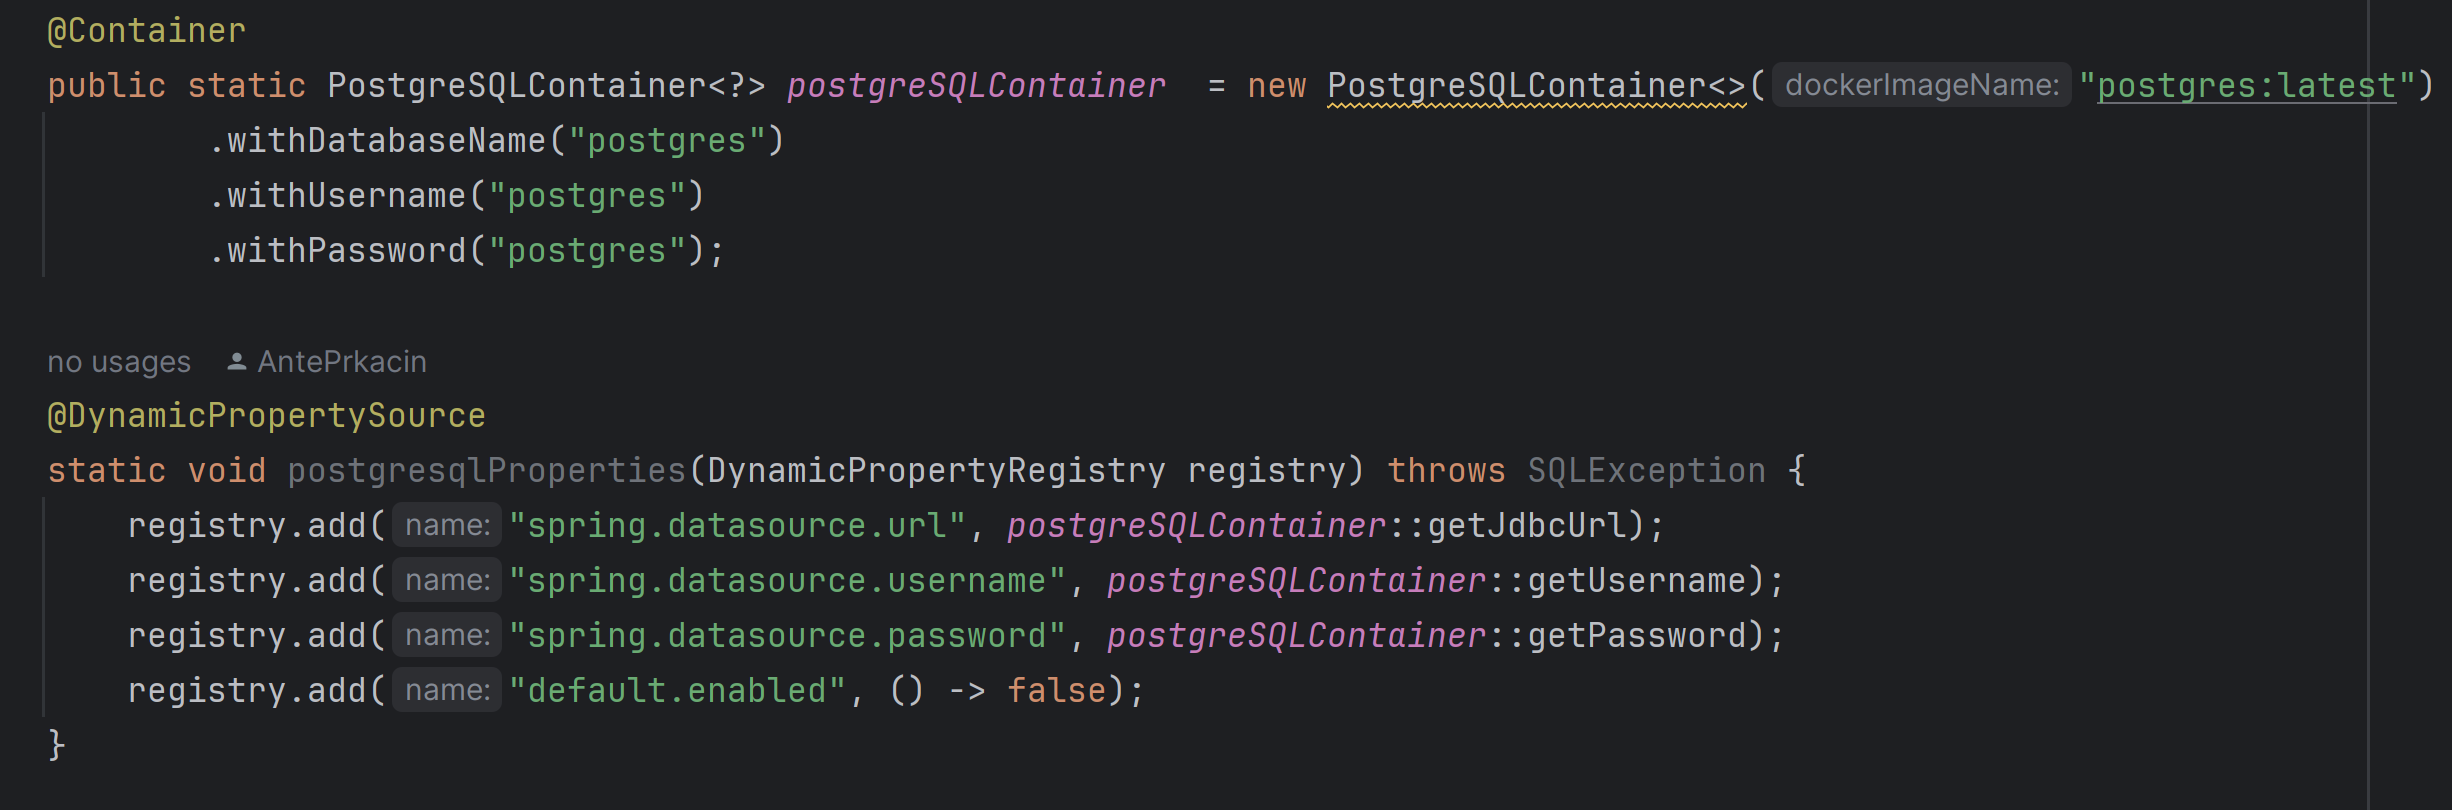
\includegraphics[scale=0.50]{slike/IT_containerized_docker.png}
                \centering
                \caption{Dizanje baze u integracijskom testu}
                \label{fig:IT_docker}
            \end{figure}

            Nakon što se baza digne, a prije pokretanja testova, izvršava se funkcija s anotacijom @BeforeEach koja u bazu umeće podatke potrebne za testiranje.
            Na primjer, ako se testira metoda za brisanje prijave, u bazu će se prije tog testa umetnuti jedna prijava.
			Ova funkcija se izvršava prije svakog testa.
            Umetanje u bazu funkcionira tako da se napravi String varijabla koja je jednaka SQL naredbi.
			Potom se izgradi objekt koji se želi umetnuti u bazu i u SQL naredbu se upisuju atributi tog objekta.
			Na kraju se SQL naredba izvršava i podatak se upisuje u bazu (Slika \ref{fig:beforeEach}).
            \begin{figure}[H]
                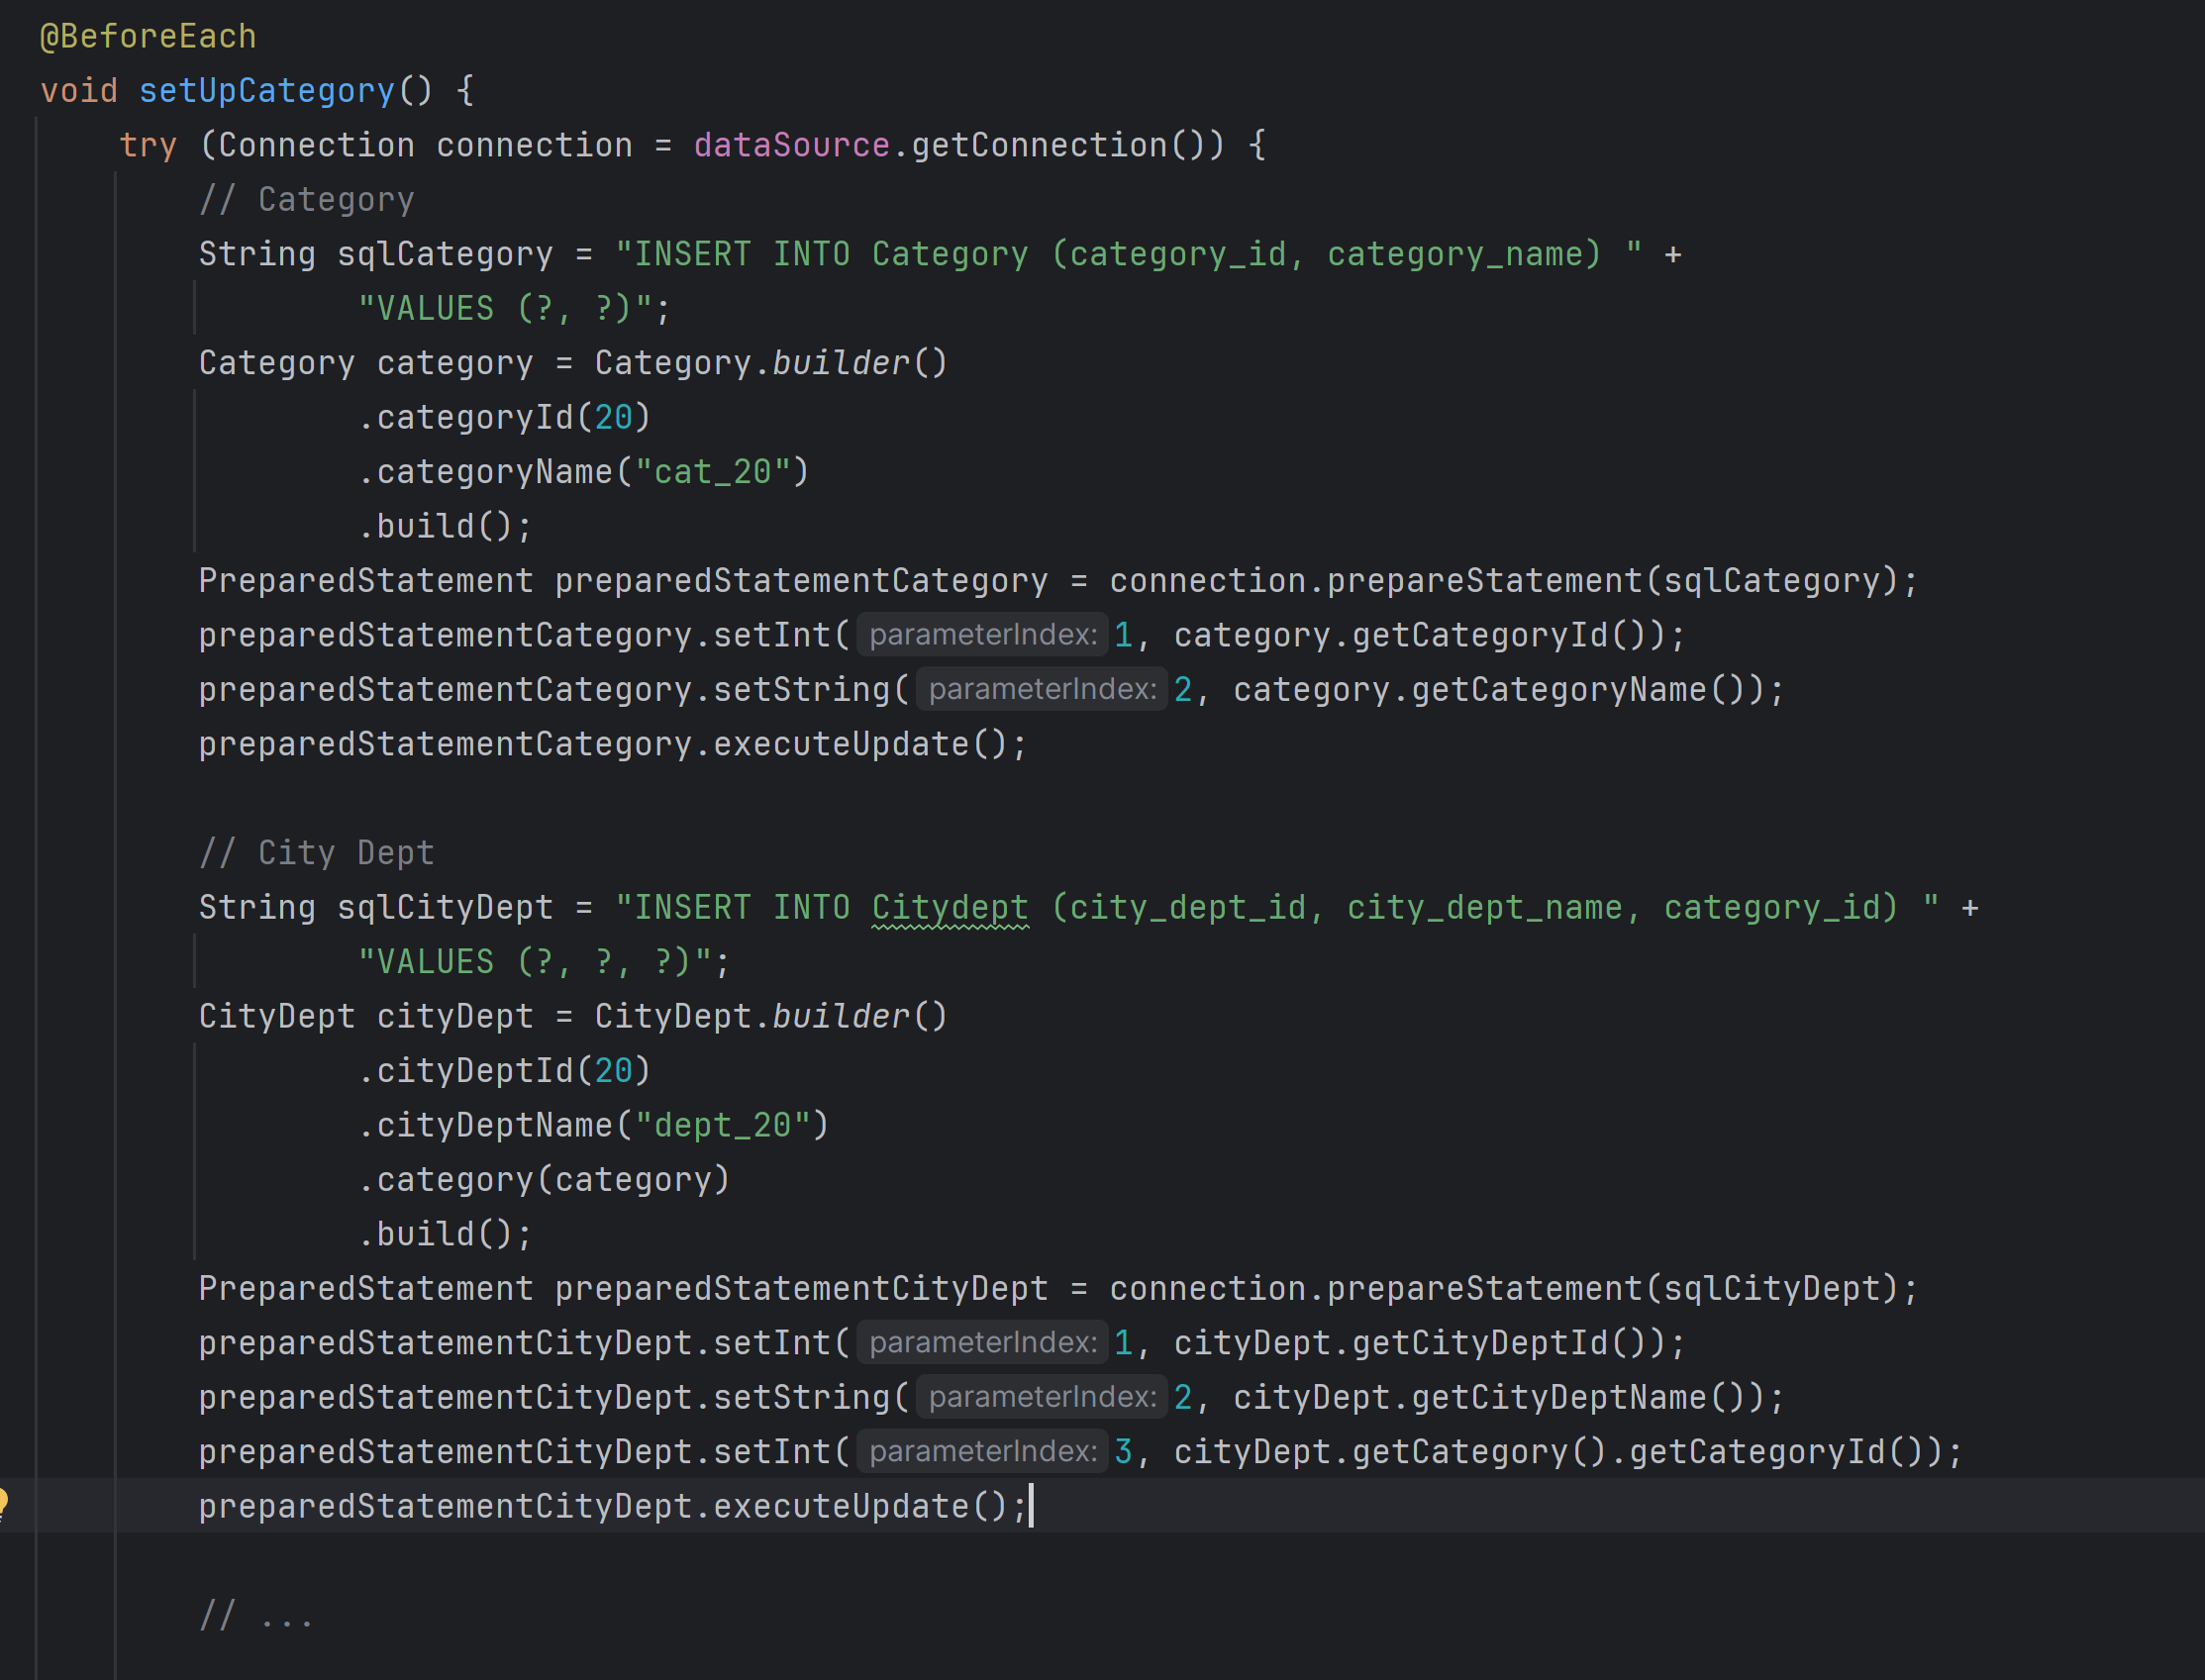
\includegraphics[scale=0.60]{slike/IT_beforeEach.png}
                \centering
                \caption{Umetanje podataka u bazu}
                \label{fig:beforeEach}
            \end{figure}

            Testovi su funkcije s anotacijom @Test.
			Za testiranje se koristi mockMvc.perform() funkcija koja simulira HTTP zahtjev, definira HTTP metodu za poziv API-a,
            predaje JSON ako treba, definira kakav contentType treba predati, je li potreban JWT za pristup API-ju i
			koji HTTP status se očekuje kao odgovor tog zahtjeva (slika \ref{fig:test}).
            \begin{figure}[H]
                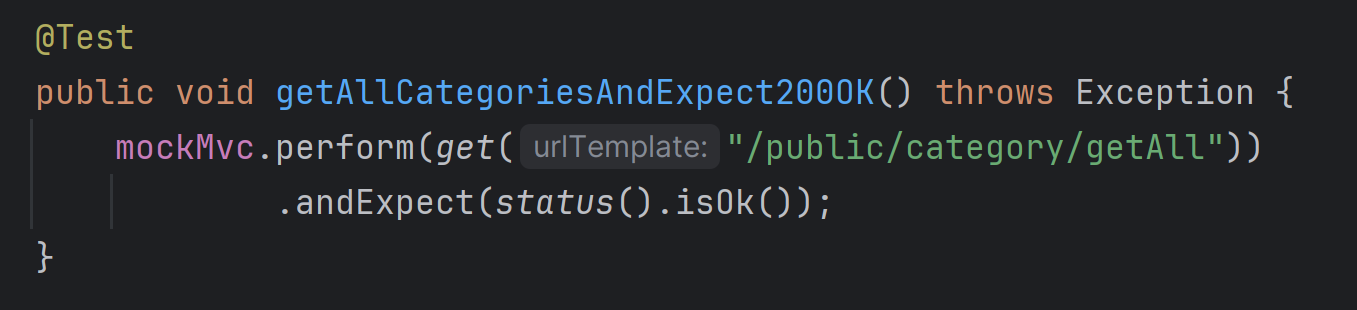
\includegraphics[scale=0.60]{slike/IT_test.png}
                \centering
                \caption{Integracijski test}
                \label{fig:test}
            \end{figure}

            Po završetku svakog testa izvršava se funkcija s anotacijom @AfterEach.
			Ona koristi JdbcTestUtils.deleteFromTables() funkciju kako bi izbrisala sve podatke iz određene tablice u bazi.
			Na ovakav način se osigurava da ako se nešto umetne u bazu prilikom testa,
			poslije završetka testa će se i izbrisati (slika \ref{fig:afterEach}).
            \begin{figure}[H]
                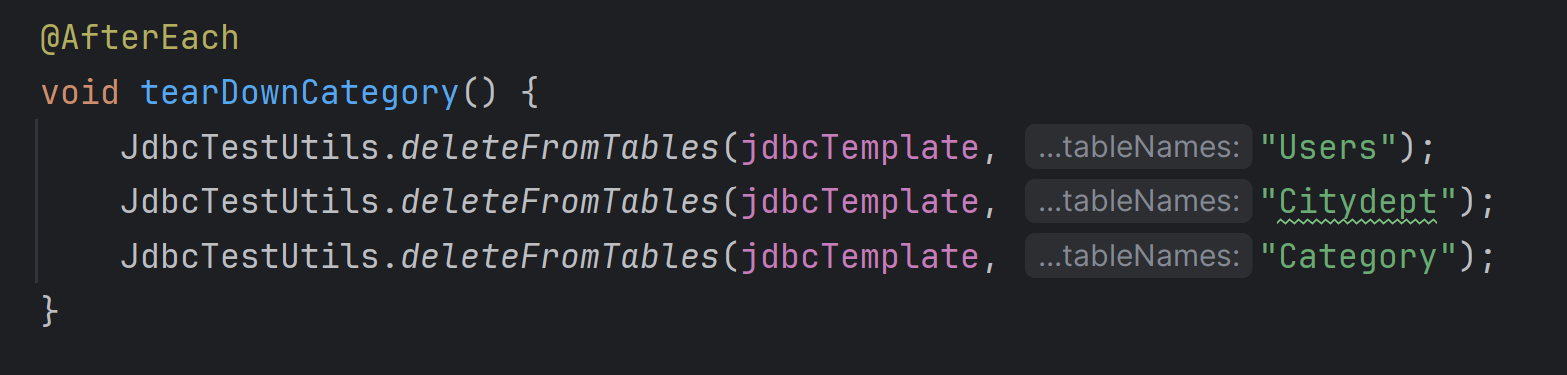
\includegraphics[scale=0.60]{slike/IT_afterEach.png}
                \centering
                \caption{Brisanje podataka iz baze nakon testa}
                \label{fig:afterEach}
            \end{figure}

            \eject
			
			\subsection{Ispitivanje sustava}

			Ispitiavanje funkcionalnosti sustava je provedeno pomoću Selenium tekstova
			pisanih i jeziku JavaScript uz preglednik Google Chrome. Ukupno je napisano
			8 testova od kojih 3 provjerava kako se sustav nosi sa pogrešnim unosima.
			 \\
			\textbf{1. Ispitni slučaj: Prijava korisnika}
			 \begin{itemize}
				\item \textbf{Ulaz:} Email adresa i lozinka korisnika 
				\item \textbf{Očekivani izlaz:} Nakon prijave nalazit ćemo se na početnoj stranici sa korisničkim imenom prikazanim u gornjem desnom kutu.
				\item \textbf{Koraci:} 
				\\ 1. Klik na gumb Login/Register
				\\ 2. Unos korisničnih podataka, točnije emaila i lozinke
				\\ 3. Klik na gumb Prijava
			\end{itemize}

			\begin{verbatim}
				const { By, Key, Builder, until } = require("selenium-webdriver");

				async function prijava() {
				let driver = await new Builder().forBrowser("chrome").build();
				try {
					await driver.get("https://cestafix-fe.onrender.com/");
					const buttonElement = await driver.findElement(By.css('#login'));
					await buttonElement.click();
					const usernameField = await driver.findElement(By.css('#username'));
					await usernameField.sendKeys('filip.simunovic@gmail.com');
					const passwordField = await driver.findElement(By.css('#password'));
					await passwordField.sendKeys('Simiklimi.5');
					const submitButton = await driver.findElement(By.css('#submit'));
					await submitButton.click();
					await driver.sleep(10000);
				} catch (error) {
					console.error("Test failed:", error);
				} finally {
					// Quit the driver
					console.log("Test je prosao uspjesno.");
					await driver.quit();
				}
				}

				prijava();
			\end{verbatim}

			\textbf{2. Ispitni slučaj: Registracija korisnika}
			 \begin{itemize}
				\item \textbf{Ulaz:} Ime, prezime, email i lozinka korisnika
				\item \textbf{Očekivani izlaz:} Nakon uspješne registracije nalazit ćemo se na početnoj stranici sa korisničkim imenom prikazanim u gornjem desnom kutu.
				\item \textbf{Koraci:} 
				\\ 1. Klik na gumb Login/Register
				\\ 2. Klik na link "Nemaš račun? Registriraj se!"
				\\ 3. Unos korisničnih podataka
				\\ 4. Klik na gumb Registriraj se
			\end{itemize}

			\begin{verbatim}
				const { By, Key, Builder, until } = require("selenium-webdriver");


				async function register() {
					let driver = await new Builder().forBrowser("chrome").build();
				  try {
					await driver.get("https://cestafix-fe.onrender.com/");
					const buttonElement = await driver.findElement(By.css('#login'));
					await buttonElement.click();
					const registerElement = await driver.findElement(By.css('#nemaracun'));
					await registerElement.click();
					const imeField = await driver.findElement(By.css('#imeid'));
					await imeField.sendKeys('Da');
					const prezimeField = await driver.findElement(By.css('#prezimeid'));
					await prezimeField.sendKeys('Vinki');
					const emailField = await driver.findElement(By.css('#emailid'));
					await emailField.sendKeys('da.vinki@gmail.com');
					const passwordField = await driver.findElement(By.css('#passwordid'));
					await passwordField.sendKeys('Vinki.66');
					const passwordrepeatField = await driver.findElement(By.css('#repatpasswordid'));
					await passwordrepeatField.sendKeys('Vinki.66');
					const submitField = await driver.findElement(By.css('#signupid'));
					await submitField.click();
					await driver.sleep(10000);
				  } catch (error) {
					console.error("Test failed:", error);
				  } finally {
					// Quit the driver
					console.log("Test je prosao uspjesno.");
					await driver.quit();
				  }
				
				}
				
				register();				
			\end{verbatim}

			\textbf{3. Ispitni slučaj: Neuspjela prijava korisnika}
			 \begin{itemize}
				\item \textbf{Ulaz:} Email adresa i \textit{netočna} lozinka korisnika
				\item \textbf{Očekivani izlaz:} Nakon unosa pogrešne lozinke korisniku se trebaju ispisati da su uneseni krivi podatci u istom prozoru.
				\item \textbf{Koraci:} 
				\\ 1. Klik na gumb Login/Register
				\\ 2. Unos korisničnih podataka, točnije emaila i lozinke
				\\ 3. Klik na gumb Prijava
			\end{itemize}

			\begin{verbatim}
				const { By, Key, Builder, until } = require("selenium-webdriver");

				async function prijava() {
				let driver = await new Builder().forBrowser("chrome").build();
				try {
					await driver.get("https://cestafix-fe.onrender.com/");
					const buttonElement = await driver.findElement(By.css('#login'));
					await buttonElement.click();
					const usernameField = await driver.findElement(By.css('#username'));
					await usernameField.sendKeys('filip.simunovic@gmail.com');
					const passwordField = await driver.findElement(By.css('#password'));
					await passwordField.sendKeys('Simiklimiii.5');
					const submitButton = await driver.findElement(By.css('#submit'));
					await submitButton.click();
					await driver.sleep(10000);
				} catch (error) {
					console.error("Test failed:", error);
				} finally {
					// Quit the driver
					console.log("Test je prosao uspjesno.");
					await driver.quit();
				}
				}

			prijava();
			\end{verbatim}

			\textbf{4. Ispitni slučaj: Registracija korisnika i brisanje računa}
			 \begin{itemize}
				\item \textbf{Ulaz:} Ime, prezime, email i lozinka korisnika
				\item \textbf{Očekivani izlaz:} Nakon registriranja i brisanja računa, ako se pokušamo logirati sa istim podatcima dobit ćemo neuspjelu prijavu.
				\item \textbf{Koraci:} 
				\\ 1. Klik na gumb Login/Register
				\\ 2. Klik na link "Nemaš račun? Registriraj se!"
				\\ 3. Unos korisničnih podataka
				\\ 4. Klik na gumb Registriraj se
				\\ 5. Klik na gumb koji prikazuje ime korisnika
				\\ 6. Klik na gumb Pobriši račun!!!
				\\ 7. Klik na gumb POTVRDI
				\\ 8. Klik na gumb Login/Register
				\\ 9. Unos korisničnih podataka
				\\ 10. Klik na gumb Prijava
			\end{itemize}

			\begin{verbatim}
				const { By, Key, Builder, until } = require("selenium-webdriver");

				async function register() {
					let driver = await new Builder().forBrowser("chrome").build();
				try {
					await driver.get("https://cestafix-fe.onrender.com/");
					const buttonElement = await driver.findElement(By.css('#login'));
					await buttonElement.click();
					const registerElement = await driver.findElement(By.css('#nemaracun'));
					await registerElement.click();
					const imeField = await driver.findElement(By.css('#imeid'));
					await imeField.sendKeys('Da');
					const prezimeField = await driver.findElement(By.css('#prezimeid'));
					await prezimeField.sendKeys('Vinki');
					const emailField = await driver.findElement(By.css('#emailid'));
					await emailField.sendKeys('da.vinkiiiiiiiii@gmail.com');
					const passwordField = await driver.findElement(By.css('#passwordid'));
					await passwordField.sendKeys('Vinkii.66');
					const passwordrepeatField = await driver.findElement
					(By.css('#repatpasswordid'));
					await passwordrepeatField.sendKeys('Vinkii.66');
					const submitField = await driver.findElement(By.css('#signupid'));
					await submitField.click();
					await driver.sleep(5000);
					const accountField = await driver.findElement(By.css("#account"));
					await accountField.click();
					await driver.sleep(2000);
					const deleteField = await driver.findElement(By.css("#brisiid"));
					await deleteField.click();
					await driver.sleep(2000);
					const delete2Field = await driver.findElement(By.css("#brisiaccid"));
					await delete2Field.click();
					await driver.sleep(2000);
					const loginButtonElement = await driver.findElement(By.css('#login'));
					await loginButtonElement.click();
					const username2Field = await driver.findElement(By.css('#username'));
					await username2Field.sendKeys('da.vinkiiiiiiiii@gmail.com');
					const password2Field = await driver.findElement(By.css('#password'));
					await password2Field.sendKeys('Vinkii.66');
					const submit2Button = await driver.findElement(By.css('#submit'));
					await submit2Button.click();
					await driver.sleep(5000);
				} catch (error) {
					console.error("Test failed:", error);
				} finally {
					// Quit the driver
					console.log("Test je prosao uspjesno.");
					await driver.quit();
				}
				}
				register();
			\end{verbatim}

			\textbf{5. Ispitni slučaj: Prijava štete anonimnog korisnika}
			 \begin{itemize}
				\item \textbf{Ulaz:} Naziv štete, opis štete, adresa štete
				\item \textbf{Očekivani izlaz:} Nakon uspješne prijave izbacit će se prozor da id-jem prijave pomoću kojeg možemo pratiti istu.
				\item \textbf{Koraci:} 
				\\ 1. Klik na gumb Prijavi Štetu!
				\\ 2. Unos podataka prijave
				\\ 3. Klik na gumb Submit
			\end{itemize}

			\begin{verbatim}
				const { By, Key, Builder, until } = require("selenium-webdriver");

				async function prijava() {
				let driver = await new Builder().forBrowser("chrome").build();
				try {
					await driver.get("https://cestafix-fe.onrender.com/");
					const buttonElement = await driver.findElement(By.css('#prijava'));
					await buttonElement.click();
					const nameField = await driver.findElement(By.css('#name'));
					await nameField.sendKeys('Palo stup na kolnik');
					const descriptionField = await driver.findElement(By.css('#description'));
					await descriptionField.sendKeys('Pao STOP znak tamo di hodaju ljudi');
					const addressField = await driver.findElement(By.css('#address'));
					await addressField.sendKeys('Unska 4');
					const submitButton = await driver.findElement(By.css('.confirmButton'));
					await submitButton.click();
					await driver.sleep(40000);
					const confirmButton = await driver.findElement(By.css('.loginbtn'));
					await confirmButton.click();
				} catch (error) {
					console.error("Test failed:", error);
				} finally {
					// Quit the driver
					console.log("Test je prosao uspjesno.");
					await driver.quit();
				}
				}
				prijava();
			\end{verbatim}


			\textbf{6. Ispitni slučaj: Prijava štete prijavljenog korisnika}
			 \begin{itemize}
				\item \textbf{Ulaz:} Email adresa i lozinka korisnika, naziv štete, opis štete, adresa štete
				\item \textbf{Očekivani izlaz:} Nakon uspješne prijave izbacit će se prozor da id-jem prijave pomoću kojeg možemo pratiti istu.
				\item \textbf{Koraci:} 
				\\ 1. Klik na gumb Login/Register
				\\ 2. Unos korisničnih podataka
				\\ 3. Klik na gumb Prijava
				\\ 4. Klik na gumb Prijavi Štetu!
				\\ 5. Unos podataka prijave
				\\ 6. Klik na gumb Submit
			\end{itemize}

			\begin{verbatim}
				const { By, Key, Builder, until } = require("selenium-webdriver");

				async function prijava() {
				let driver = await new Builder().forBrowser("chrome").build();
				try {
					await driver.get("https://cestafix-fe.onrender.com/");
					const buttonElement = await driver.findElement(By.css('#login'));
					await buttonElement.click();
					const usernameField = await driver.findElement(By.css('#username'));
					await usernameField.sendKeys('filip.simunovic@gmail.com');
					const passwordField = await driver.findElement(By.css('#password'));
					await passwordField.sendKeys('Simiklimi.5');
					const submitButton = await driver.findElement(By.css('#submit'));
					await submitButton.click();
					await driver.sleep(5000);
					// prijava
					const button2Element = await driver.findElement(By.css('#prijava'));
					await button2Element.click();
					const nameField = await driver.findElement(By.css('#name'));
					await nameField.sendKeys('Palo stup na kolnik opet');
					const descriptionField = await driver.findElement(By.css('#description'));
					await descriptionField.sendKeys('Pao js jedan 
					STOP znak tamo di hodaju ljudi');
					const addressField = await driver.findElement(By.css('#address'));
					await addressField.sendKeys('Unska 5');
					const submit2Button = await driver.findElement(By.css('.confirmButton'));
					await submit2Button.click();
					await driver.sleep(40000);
				} catch (error) {
					console.error("Test failed:", error);
				} finally {
					// Quit the driver
					console.log("Test je prosao uspjesno.");
					await driver.quit();
				}
				}

				prijava();
			\end{verbatim}


			
			\textbf{7. Ispitni slučaj: Neuspjela registracija korisnika}
			 \begin{itemize}
				\item \textbf{Ulaz:} Ime, prezime, email i \text{neispravna lozinka} (ne zadovoljava uvijet da mora biti dugačka 8 znakova, imati jedno veliko, jedno malo slovo, jedan broj i jedan specijalan znak) korisnika
				\item \textbf{Očekivani izlaz:} Nakon neuspješne registracije korisniku će se ispitati kako lozinka ne zadovoljava sigurnosni uvijet.
				\item \textbf{Koraci:} 
				\\ 1. Klik na gumb Login/Register
				\\ 2. Klik na link "Nemaš račun? Registriraj se!"
				\\ 2. Unos korisničnih podataka
				\\ 3. Klik na gumb Registriraj se
			\end{itemize}

			\begin{verbatim}
					const { By, Key, Builder, until } = require("selenium-webdriver");

				// Test sa neispravnom lozinkom
				async function register() {
					let driver = await new Builder().forBrowser("chrome").build();
				try {
					await driver.get("https://cestafix-fe.onrender.com/");
					const buttonElement = await driver.findElement(By.css('#login'));
					await buttonElement.click();
					const registerElement = await driver.findElement(By.css('#nemaracun'));
					await registerElement.click();
					const imeField = await driver.findElement(By.css('#imeid'));
					await imeField.sendKeys('Da');
					const prezimeField = await driver.findElement(By.css('#prezimeid'));
					await prezimeField.sendKeys('Vinki');
					const emailField = await driver.findElement(By.css('#emailid'));
					await emailField.sendKeys('da.vinki@gmail.com');
					const passwordField = await driver.findElement(By.css('#passwordid'));
					await passwordField.sendKeys('Vinki.5');
					const passwordrepeatField = await driver.findElement
					(By.css('#repatpasswordid'));
					await passwordrepeatField.sendKeys('Vinki.5');
					const submitField = await driver.findElement(By.css('#signupid'));
					await submitField.click();
					await driver.sleep(10000);
				} catch (error) {
					console.error("Test failed:", error);
				} finally {
					// Quit the driver
					console.log("Test je prosao uspjesno.");
					await driver.quit();
				}
				}
				register();
			\end{verbatim}

			\textbf{8. Ispitni slučaj: Neuspjela prijava štete logiranog korisnika}
			 \begin{itemize}
				\item \textbf{Ulaz:} Podatci prijave \textit{bez} podatka o lokaciji
				\item \textbf{Očekivani izlaz:} Nakon što nije unesena nikakva lokacija, korisniku će se u prozoru prikazati ispis "Došlo je do greške, provjerite unos adrese prijave!"
				\item \textbf{Koraci:} 
				\\ 1. Klik na gumb Login/Register
				\\ 2. Unos korisničnih podataka
				\\ 3. Klik na gumb Prijava
				\\ 4. Klik na gumb Prijavi Štetu!
				\\ 5. Unos podataka prijave
				\\ 6. Klik na gumb Submit
			\end{itemize}

			\begin{verbatim}
				const { By, Key, Builder, until } = require("selenium-webdriver");

			// report bez unosa lokacije - error
			async function prijava() {
			let driver = await new Builder().forBrowser("chrome").build();
			try {
				await driver.get("https://cestafix-fe.onrender.com/");
				const buttonElement = await driver.findElement(By.css('#login'));
				await buttonElement.click();
				const usernameField = await driver.findElement(By.css('#username'));
				await usernameField.sendKeys('filip.simunovic@gmail.com');
				const passwordField = await driver.findElement(By.css('#password'));
				await passwordField.sendKeys('Simiklimi.5');
				const submitButton = await driver.findElement(By.css('#submit'));
				await submitButton.click();
				await driver.sleep(5000);
				// prijava
				const button2Element = await driver.findElement(By.css('#prijava'));
				await button2Element.click();
				const nameField = await driver.findElement(By.css('#name'));
				await nameField.sendKeys('Palo stup na kolnik opet');
				const descriptionField = await driver.findElement(By.css('#description'));
				await descriptionField.sendKeys('Pao js jedan STOP znak tamo di hodaju ljudi');
				const submit2Button = await driver.findElement(By.css('.confirmButton'));
				await submit2Button.click();
				await driver.sleep(40000);
			} catch (error) {
				console.error("Test failed:", error);
			} finally {
				// Quit the driver
				console.log("Test je prosao uspjesno.");
				await driver.quit();
			}
			}
			prijava();
			\end{verbatim}

			
			\eject 
		
		\section{Dijagram razmještaja}
			
			Dijagram razmještaja opisuje topologiju sustava i usredotočen je na odnos sklopovskih i programskih
			dijelova. Prikazan je na slici 5.1. Na poslužiteljskom računalu se nalazi Render servis, Frontend HTTP poslužitelj, Backend HTTP 
			poslužitelj te PostgreSQL poslužitelj na kojem je baza podataka. Na Frontend HTTP poslužitelju se nalazi
			React frontend CestaFix aplikacije. Na Backend HTTP poslužitelju se nalazi ReportApplication.jar, tj. 
			Java Archive file u kojem se nalazi backend CestaFix aplikacije. Poslužiteljska strana aplikacije
			ostvarena je pomoću servisa Render. Klijenti koriste web preglednik kako bi pristupili web aplikaciji. 
			Sustav je baziran na arhitekturi "klijent - poslužitelj", a komunikacija između računala korisnika
			i poslužitelja odvija se preko HTTP veze.

			\begin{figure}[H]
				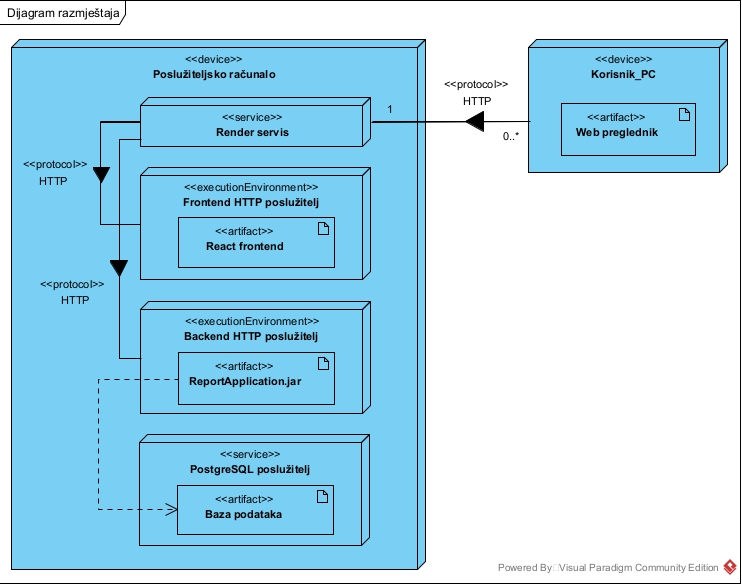
\includegraphics[scale=0.60]{slike/DR.jpg} %veličina slike u odnosu na originalnu datoteku i pozicija slike
				\centering
				\caption{Dijagram razmještaja}
				\label{fig:DijagramRazmjestaja}
			\end{figure}

			\eject 
		
		\section{Upute za puštanje u pogon}

			Za pogon naše aplikacije korištena je platforma Render koja pruža besplatno puštanje aplikacije u pogon sa, naravno, ograničenim mogućnostima.   

			\subsection{Puštanje baze podataka u pogon} 
			Prvo je potrebno upogoniti bazu podataka. Nakon prijavljivanja u platformu, potrebno je odabrati opciju New \texttt{->} PostgreSQL slika \ref{fig:Kreiranjenovogservisa}. 
			Zatim je na ekranu prikazan unos podataka za bazu podataka, za što smo mi ostavili sve prazno (automatski se generira) osim imena servisa, te je za regiju potrebno postaviti \texttt{Frankfurt(EU Central)} slika \ref{fig:Unos podataka za bazu}.
			Nedostatak besplatne verzije Rendera je to što je moguća samo jedna baza podataka koja je ograničena na trajanje od 3 mjeseca, no to je dovoljno za naše potrebe.
			\begin{figure}[H]
				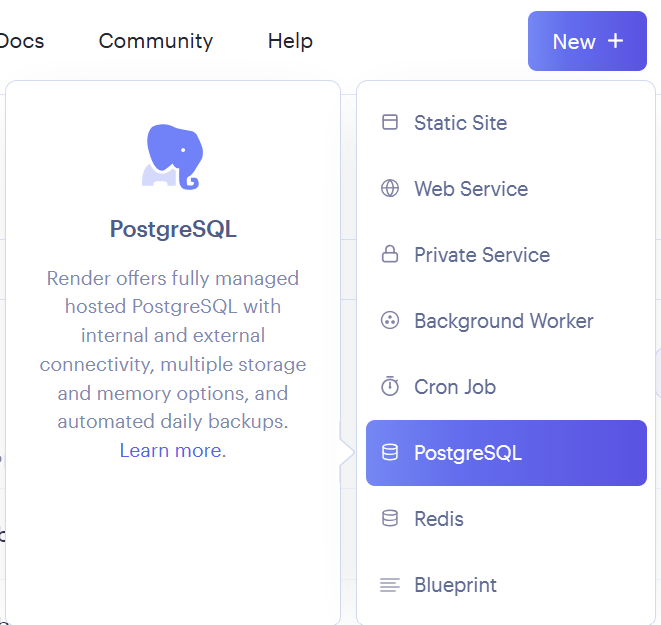
\includegraphics[scale=0.60]{slike/render1.png} %veličina slike u odnosu na originalnu datoteku i pozicija slike
				\centering
				\caption{Kreiranje novog servisa}
				\label{fig:Kreiranjenovogservisa}
			\end{figure}

			\begin{figure}[H]
				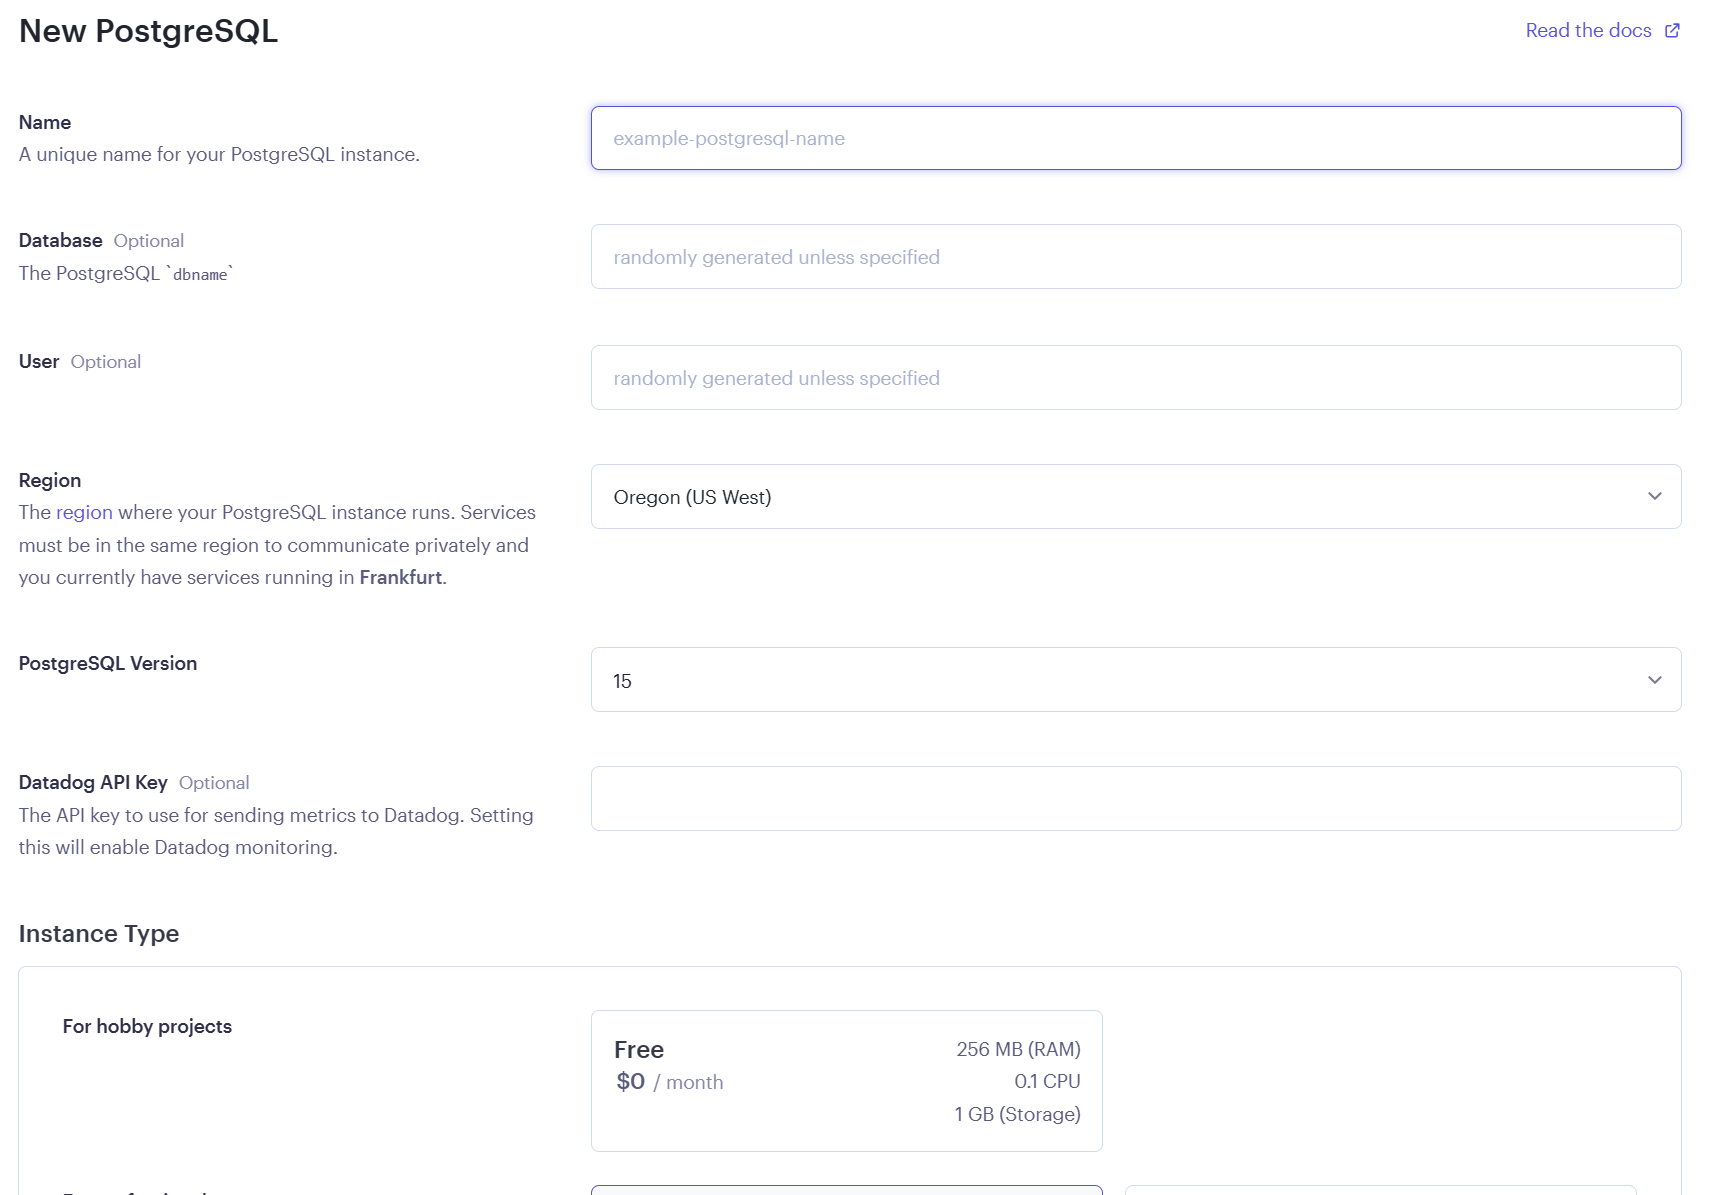
\includegraphics[scale=0.40]{slike/render2.png} %veličina slike u odnosu na originalnu datoteku i pozicija slike
				\centering
				\caption{Unos podataka za bazu}
				\label{fig:Unos podataka za bazu}
			\end{figure}

			\subsection{Puštanje backenda u pogon} 
			Isto tako je potrebno podesiti backend. Prvo je potrebno odabrati opciju \texttt{Web Service} u \ref{fig:Kreiranjenovogservisa}.
			Nakon toga imamo opciju odabrati deploy preko github repozitorija, što omogućava automatsko redeployanje svaki put kada se napravi novi commit.
			Nakon odabira našeg repozitorija, opet imamo ekran za unos podataka \ref{fig:UnosPodatakaZaBack}
			\begin{figure}[H]
				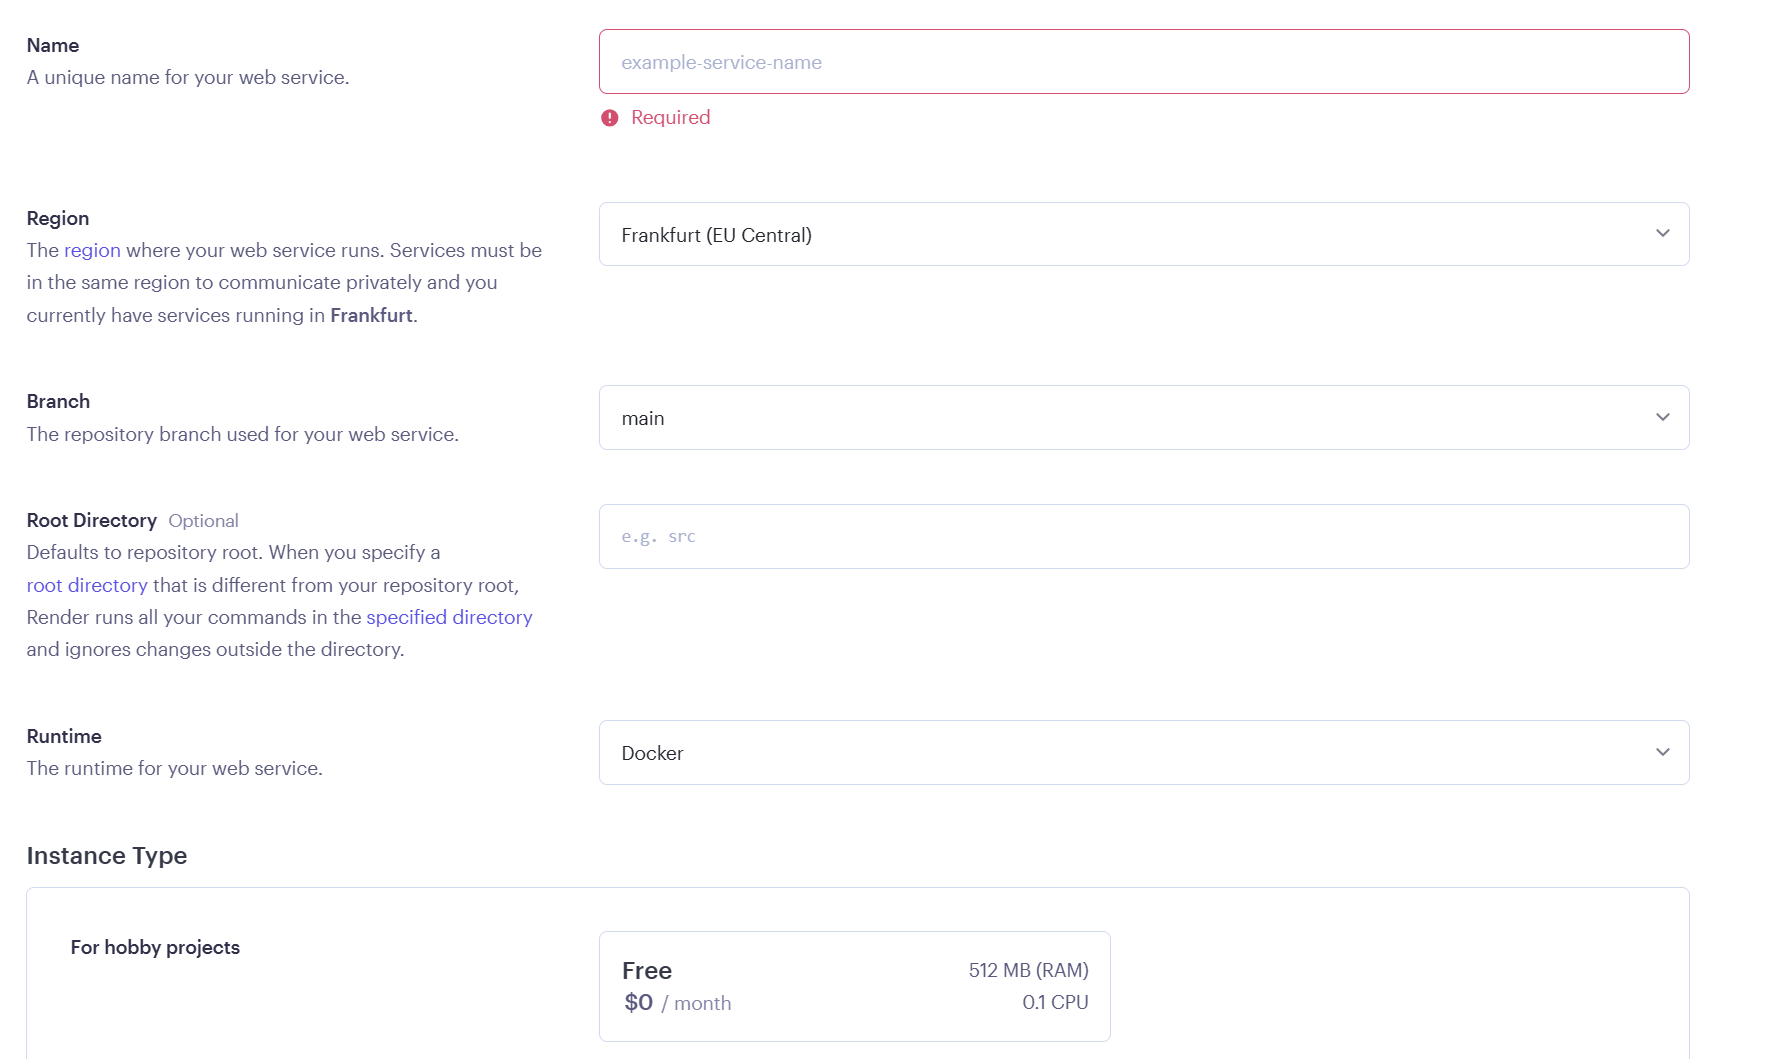
\includegraphics[scale=0.40]{slike/render3.png} %veličina slike u odnosu na originalnu datoteku i pozicija slike
				\centering
				\caption{Unos podataka za backend}
				\label{fig:UnosPodatakaZaBack}
			\end{figure}
			Za ime upisati željeno ime servisa, za regiju staviti Frankfurt, odabrati granu i pozicionirati se u backend direktorij. Za runtime staviti Docker.
			Nakon toga je potrebno upisat podatke za varijable okoline koje nam omogućavaju povezivanje na prethodno deployanu bazu \ref{fig:EnvVarijable}
			\begin{figure}[H]
				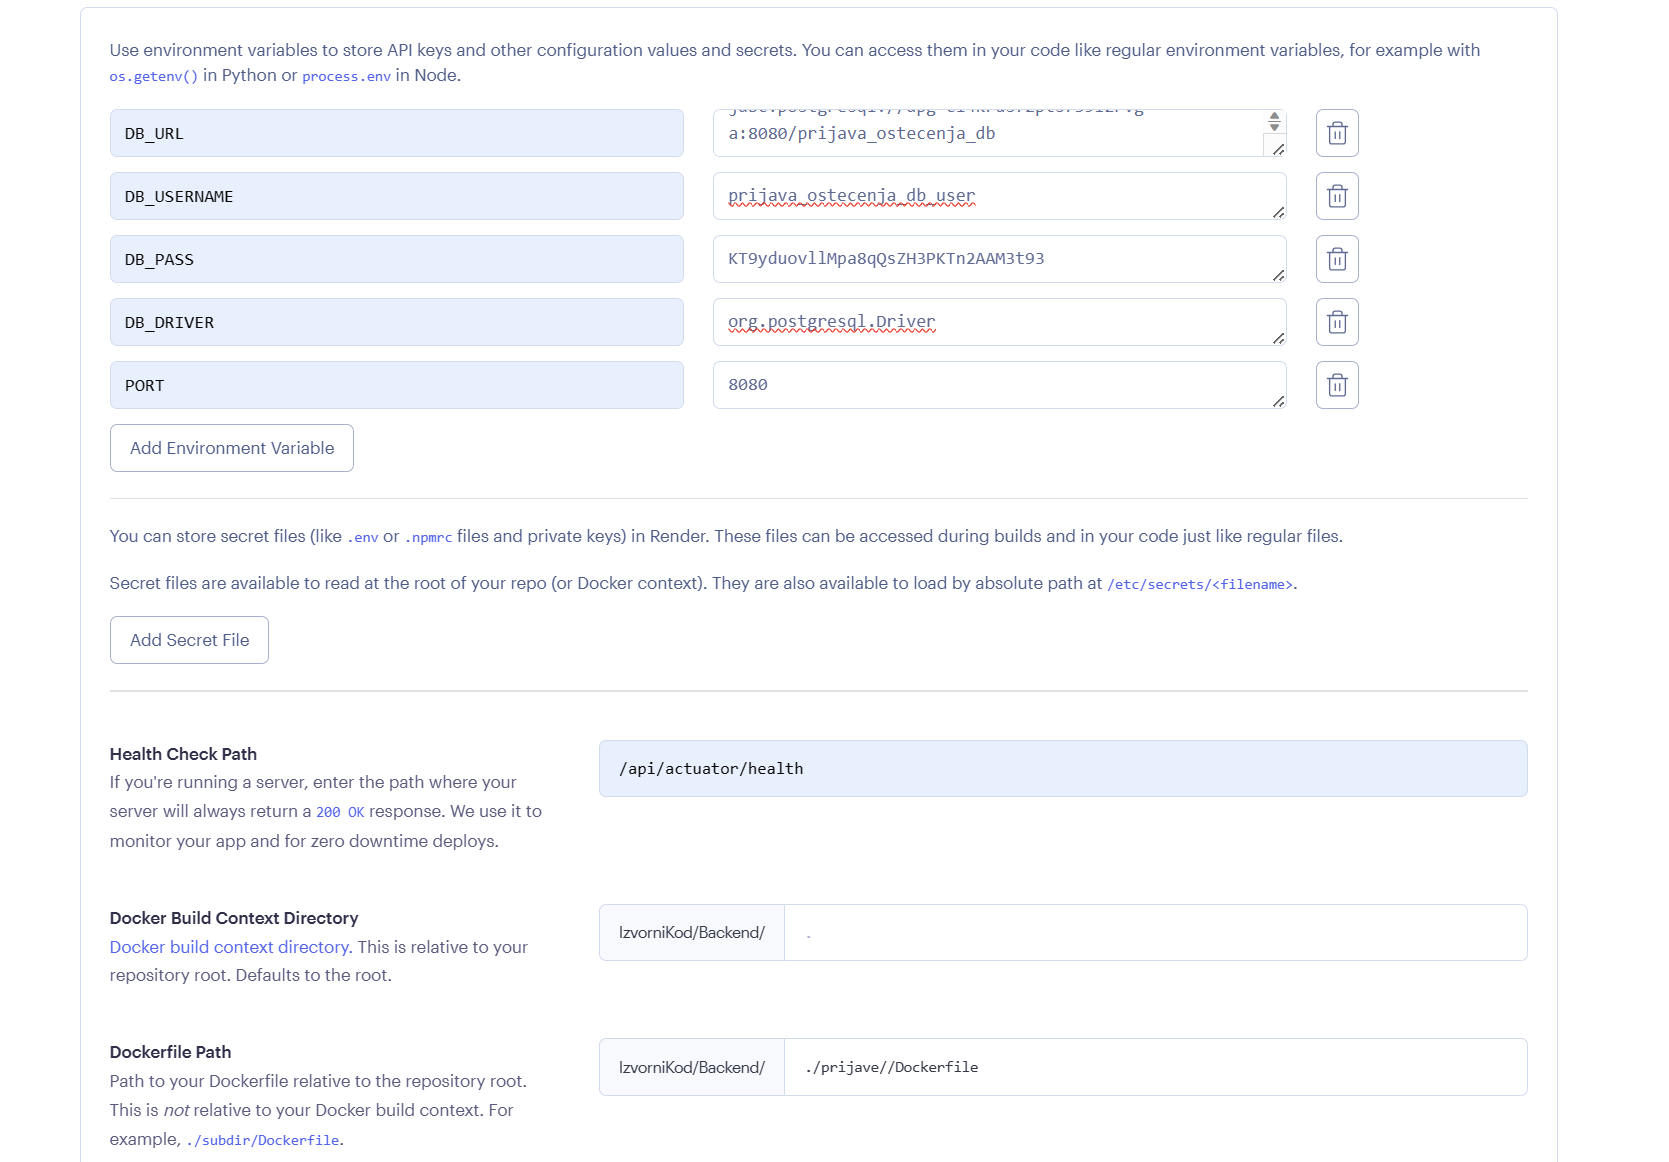
\includegraphics[scale=0.40]{slike/render4.png} %veličina slike u odnosu na originalnu datoteku i pozicija slike
				\centering
				\caption{Unos varijabli okoline za backend}
				\label{fig:EnvVarijable}
			\end{figure}

			Nakon toga je potrebno klikom na gumb Advanced pod opcijom Health Check Path upisati \texttt{api/actuator/health}, te pod Dockerfile Path odabrati Dockerfile iz repozitorija, konkretno \texttt{./prijave/Dockerfile}.
			Time bi backend trebao biti deployan.

			\subsection{Puštanje frontenda u pogon} 
			Frontend se pušta u pogon na sličan način. Potrebno je odabarti Web Service opciju \ref{fig:Kreiranjenovogservisa}, odabrati git repozitorij, upisati ime, odabrati Frankfurt, odabrati git granu i napisati putanju do frontend koda. Za runtime odabrati Node, za Build Command staviti yarn build, te za Start Command yarn start-prod.
			Time bi frontend trebao biti pušten u pogon.

			\eject 